\chapter{Non-linear Kernels} % Main chapter title

\label{Chapter1} % For referencing the chapter elsewhere, use \ref{Chapter1} 
\label{eq:ch4.grankingcoeff}

%----------------------------------------------------------------------------------------

This modification intends to apply the required modifications in the calculation of the ranking criteria so that non-linear kernels can be used in the SVM.

\section{Description and reasoning}
\label{sec:stopCond.desc}

When a problem is not linearly separable, we know that a hard-margin SVM will not be able to correctly place a decision boundary. In this case a soft-margin SVM may be used, but it only works to some extent and if the underlying distribution is near linearly separable. If it is not the case, much better results can be achieved by using non-linear kernels.

To use this method within SVM-RFE we must first be able to compute the ranking coefficient from a non-linear kernel. In contrast with the linear kernel case, where the ranking coefficient can be simplified to $(w_i)^2$, for non-linear kernels, however, since it is a more general case, no simplification can be performed. Instead, we use the general ranking coefficient for SVM (Equation \ref{eq:ch4.grankingcoeff}), which we restate here:
\begin{align*}
    DJ(i) = (1/2)(\boldsymbol{\alpha}^\T \vb{H} \boldsymbol{\alpha} - \boldsymbol{\alpha}^\T \vb{H}(-i) \boldsymbol{\alpha})
\end{align*}

Note that the \emph{hessian} matrix $\vb{H_{i,j}} = y_iy_jk(\vb{x_i}, \vb{x_j})$ needs be computed each iteration (since the dimension of $\vb{x_i}$ and $\vb{x_j}$ will change), and also for each feature removed in each iteration. This is slow. However, various optimizations may exist, as discussed in Section [ref.].

\section{Pseudocode formalization}

\textbf{Definitions:}

\begin{itemize}
    \item $X_0 = [\vt{x_0}, \vt{x_1}, \dotsc, \vt{x_k}]^T$ list of observations.
    \item $\vt{y} = [y_1, y_2, \dotsc, y_k]^T$ list of labels.
\end{itemize}

\begin{algorithm}[H]
    \DontPrintSemicolon
      \KwInput{$t, k$ \tcp*{$t$ = step, $k$ = kernel function}}
      \KwOutput{$\vt{r}$}
      \KwData{$X_0,\vt{y}$}
      $\vt{s} = [1,2, \dotsc, n]$ \tcp*{subset of surviving features}
      $\vt{r} = []$ \tcp*{feature ranked list}
      \While{$|\vt{s}| > 0$}
        {
            \tcc*[h]{Restrict training examples to good feature indices}\\
            $X=X_0(:,\vt{s})$\VS

            \tcc*[h]{Precompute hessian matrix}\\
            $\vb{H_{i,j}} = y_iy_jk(\vb{x_i}, \vb{x_j}) \qquad \text{for all} \qquad \vb{x_i}, \vb{x_j} \in X$\VS

            \tcc*[h]{Train the classifier}\\
            $\vt{\alpha} = \texttt{SVM-train(} X, y, k \texttt{)}$\VS

            \tcc*[h]{Compute the ranking criteria}\\
            $\vt{c} = [c_1, c_2, \dots, c_{|\vt{s}|}]$ \\
            \For{$c_l \in \vt{c}$}{
                \tcc*[h]{Compute new hessian with the feature $l$ removed}\\
                $\vb{H_{i,j}}(-l) = y_iy_jk(\vb{x_i}, \vb{x_j}) \qquad \text{for all} \qquad \vb{x_i}, \vb{x_j} \in X(-l)$\VS
    
                \tcc*[h]{Calculate ranking coefficient}\\
                $c_l = (1/2)(\boldsymbol{\alpha}^\T \vb{H} \boldsymbol{\alpha} - \boldsymbol{\alpha}^\T \vb{H}(-l) \boldsymbol{\alpha})$
            }\VS

            \tcc*[h]{Find the $t$ features with the smallest ranking criterion}\\
            $\vt{f} = \texttt{argsort}(\vt{c})(\ :t)$\VS

            \tcc*[h]{Iterate over the feature subset}\\
            \For{$f_i \in \vt{f}$}{
                \tcc*[h]{Update the feature ranking list}\\
                $\vt{r} = [\vt{s}(f_i), ...\vt{r}]$\VS
    
                \tcc*[h]{Eliminate the feature selected}\\
                $\vt{s} = [...\vt{s}(1:f_i - 1), ...\vt{s}(f_i + 1:|\vt{s}|)]$
            }
        }
    \caption{SVM-RFE with general Kernel}
    \label{alg:svmrfe-stopcond}
\end{algorithm}

\section{Results}

\subsection*{Notes on the implementation}

Using non-linear kernels requires a change in the underlying implementation we've been using for SVM. Until now, we've been relying on the \texttt{LinearSVC} model pro\-vid\-ed by \texttt{Sklearn}, this implementation is in turn based on the \texttt{LIBLINEAR} im\-ple\-men\-ta\-tion for SVM written by the \emph{National Taiwan University}. The authors state that this solver is much faster than the more general version, thus the reason we've been using it, but it can only handle linear kernels. The general version, \texttt{LIBSVM}, created by the same team, is the option we're going to use instead. Because now we need to switch, it is interesting to see what will be the increase in computational cost, shown in the table \ref{ch5.kernels.tc1}.

For this first test we've generated artificial datasets with 100 features each, 20 which are informative. Because we want to test the differences with the linear kernel we've used 6 Gaussian clusters per class, this makes the problem more difficult for lineal separators. 

To obtain similar results to what we would get with SVM-RFE, we've tested under the random feature selection model (which is the same as RFE with random criteria) and made a comparison using different amount of samples.

\begin{table}[h]
    \centering
    \begin{tabular}{l c c c}
        \toprule
        Obs. & \texttt{LIBLINEAR} & \texttt{LIBSVM} \emph{Linear} & \texttt{LIBSVM} \emph{Precomputed} \\
        \midrule
        500 & 02.67s & 08.17s — x0.32 & 12.04s — x0.22 \\
        1000 & 02.94s & 17.30s — x0.17 & 23.84s — x0.12 \\
        2000 & 04.28s & 43.96s — x0.10 & 50.36s — x0.08 \\
        \bottomrule
        \end{tabular}
    \caption{Cost in time and speedup of a random selection under different implementations and sample sizes.}
    \label{ch5.kernels.tc1}
\end{table}

Note that the sample size increases the cost more than linearly, this may suggest that methods such as dynamic sampling can perform even better than with the \texttt{LIBLINEAR} implementation.

We also note that using a precomputed kernel matrix (\emph{Gramm} matrix) does affect computational cost. This is likely an implementation detail and it is not significant enough to require further in\-ves\-ti\-ga\-tion.

We can also plot some examples to compare differences in accuracy, in Figure \ref{fig:ch5.kernel.cmp1} note that the precomputed kernel, which is a degree-3 polynomial kernel, performs much better at the start, thus we can expect it to also perform significantly better with SVM-RFE. At the same time, we can appreciate some differences between the two linear kernels, but they're still clearly following the same curve, which indicates that both implementations are equivalent.  

\begin{figure}[H]
    \centering
    \begin{subfigure}[b]{0.32\linewidth}
        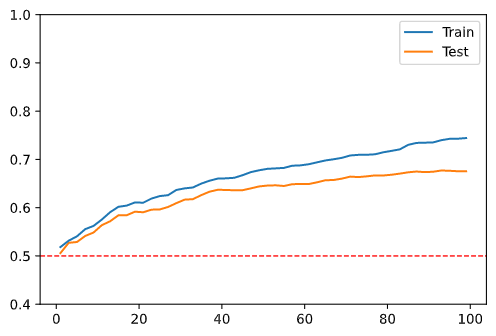
\includegraphics[width=\linewidth]{img/random_liblinarl.png}
        \subcaption*{\texttt{LIBLINEAR}}
    \end{subfigure}
    \begin{subfigure}[b]{0.32\linewidth}
        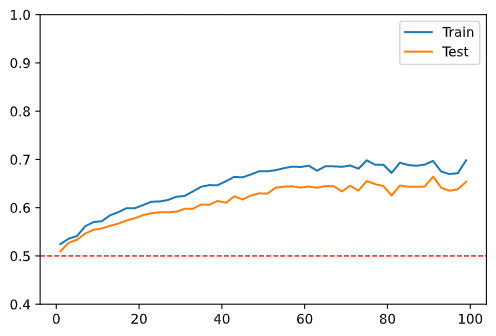
\includegraphics[width=\linewidth]{img/random_linar.png}
        \subcaption*{\texttt{LIBSVM} \emph{Linear}}
    \end{subfigure}
    \begin{subfigure}[b]{0.32\linewidth}
        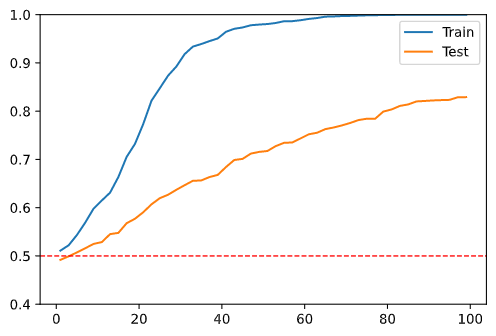
\includegraphics[width=\linewidth]{img/random_precomputed.png}
        \subcaption*{\texttt{LIBSVM} \emph{Precomputed}}
    \end{subfigure}
    \caption{Comparison of random selection with 2000 observations.}
    \label{fig:ch5.kernel.cmp1}
\end{figure}

\subsection*{Performance evaluation}

We observe experimentally in figure \ref{fig:ch5.kernel.cmp2} that, for some datasets, using a non-lineal kernel improves the accuracy of SVM-RFE.

\begin{figure}[H]
    \centering
    \begin{subfigure}[b]{0.4\linewidth}
        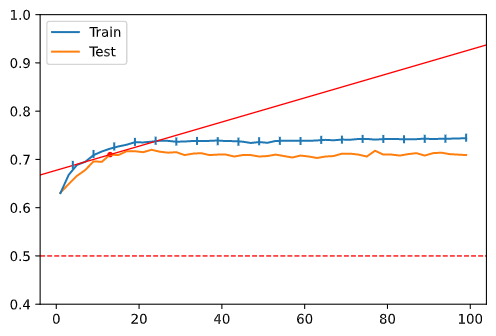
\includegraphics[width=\linewidth]{img/art_linear.png}
        \subcaption*{Linear}
    \end{subfigure}
    \begin{subfigure}[b]{0.4\linewidth}
        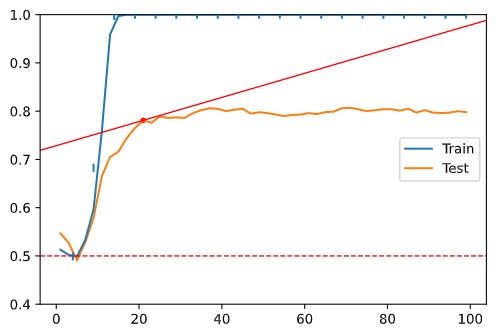
\includegraphics[width=\linewidth]{img/art_poly.png}
        \subcaption*{Poly $D=3$}
    \end{subfigure}
    \caption{Comparison of SVM-RFE on linear and non-linear kernel with 1000 observations and step of 5.}
    \label{fig:ch5.kernel.cmp2}
\end{figure}

Non-lineal kernels also involve more hyper-parameters, thus increasing the im\-por\-tance of model selection. The choice of kernel is in itself a hyper-parameter. If a polynomial kernel is chosen then the \emph{degree} and \emph{coefficient} are also hyper-parameters, if a Gaussian kernel is chosen then \emph{gamma}.

\subsection*{MADELON}

For this experiment we use the MADELON dataset with a sample of 1200 ob\-ser\-va\-tions after normalization. We're using a trade-off linear scalarization of 0.8 to determine the optimum, and a constant step of 20 and 10 for the RFE and validation phases respectively. Also, for numerical stability, all results are an average of a 6-fold cross-validation.

\subsubsection*{Polynomial}

\begin{table}[h]
    \centering
    \begin{tabular}{l | c c c|c c c|c c c}
        \toprule
        \multicolumn{1}{c}{\textbf{deg.}} & \multicolumn{3}{c}{\textbf{1}} & \multicolumn{3}{c}{\textbf{2}} & \multicolumn{3}{c}{\textbf{3}}\\
        %\cline{2-4}\cline{5-7}\cline{8-10}
        \midrule
        \textbf{C}&Feat.&Acc.&Cost&Feat.&Acc.&Cost&Feat.&Acc.&Cost \\
        \midrule
        \textbf{0.1}&      11 & 58.92\% & 0.333 &      21 & 69.08\% & 0.256 &    21 & 74.25\% & 0.214\\
        \textbf{0.2}&      1  & 61.33\% & 0.310 &      21 & 69.17\% & 0.255 &    21 & 76.58\% & 0.196\\
        \textbf{0.3}&      1  & 61.42\% & 0.309 &      21 & 70.17\% & 0.247 &    21 & 77.08\% & 0.191\\
        \textbf{0.4}&      1  & 61.33\% & 0.310 &      21 & 70.92\% & 0.241 &    21 & 77.42\% & 0.189\\
        \textbf{0.5}&      11 & 61.42\% & 0.313 &      21 & 70.83\% & 0.242 &    21 & 78.33\% & 0.182\\
        \textbf{0.6}&      1  & 61.25\% & 0.310 &      21 & 71.00\% & 0.240 &    21 & 78.00\% & 0.184\\
        \textbf{0.7}&      1  & 61.08\% & 0.312 &      21 & 70.58\% & 0.244 &    21 & 77.50\% & 0.188\\
        \textbf{0.8}&      1  & 61.25\% & 0.310 &      21 & 70.00\% & 0.248 &    21 & 76.92\% & 0.193\\
        \textbf{0.9}&      1  & 61.08\% & 0.312 &      21 & 70.00\% & 0.248 &    21 & 78.42\% & 0.181\\
        \bottomrule
        \toprule
        \multicolumn{1}{c}{\textbf{deg.}} & \multicolumn{3}{c}{\textbf{4}} & \multicolumn{3}{c}{\textbf{5}} & \multicolumn{3}{c}{\textbf{6}}\\
        %\cline{2-4}\cline{5-7}\cline{8-10}
        \midrule
        \textbf{C}&Feat.&Acc.&Cost&Feat.&Acc.&Cost&Feat.&Acc.&Cost \\
        \midrule
        \textbf{0.1}&      21 & 72.83\% & 0.226 &      21 & 70.58\% & 0.244 &    21 & 67.17\% & 0.271\\
        \textbf{0.2}&      21 & 80.92\% & 0.161 &      21 & 78.08\% & 0.184 &    21 & 77.75\% & 0.186\\
        \textbf{0.3}&      21 & 81.92\% & 0.153 &      21 & 83.92\% & 0.137 &    21 & 81.67\% & 0.155\\
        \textbf{0.4}&      21 & 82.75\% & 0.146 &      21 & 84.75\% & 0.130 &    21 & 83.58\% & 0.140\\
        \textbf{0.5}&      21 & 83.08\% & 0.144 &      21 & 84.75\% & 0.130 &    21 & 85.84\% & 0.122\\
        \textbf{0.6}&      21 & 84.00\% & 0.136 &      21 & 85.75\% & 0.122 &    21 & 84.16\% & 0.135\\
        \textbf{0.7}&      21 & 82.92\% & 0.145 &      21 & 85.50\% & 0.124 &    21 & 84.08\% & 0.132\\
        \textbf{0.8}&      21 & 83.75\% & 0.138 &      21 & 85.42\% & 0.125 &    21 & 86.16\% & 0.115\\
        \textbf{0.9}&      21 & 84.33\% & 0.138 &      \mrk{21} & \mrk{86.83\%} & \mrk{0.114} &    21 & 84.08\% & 0.132\\
        \bottomrule
        \toprule
        \multicolumn{1}{c}{\textbf{deg.}} & \multicolumn{3}{c}{\textbf{7}} & \multicolumn{3}{c}{\textbf{8}} & \multicolumn{3}{c}{\textbf{9}}\\
        %\cline{2-4}\cline{5-7}\cline{8-10}
        \midrule
        \textbf{C}&Feat.&Acc.&Cost&Feat.&Acc.&Cost&Feat.&Acc.&Cost \\
        \midrule
        \textbf{0.1}&      11 & 66.33\% & 0.274 &      11 & 64.92\% & 0.285 &    11 & 63.25\% & 0.298\\
        \textbf{0.2}&      11 & 69.17\% & 0.251 &      11 & 57.33\% & 0.345 &    11 & 56.67\% & 0.351\\
        \textbf{0.3}&      11 & 70.75\% & 0.238 &      11 & 55.17\% & 0.363 &    11 & 51.50\% & 0.392\\
        \textbf{0.4}&      11 & 83.00\% & 0.140 &      11 & 58.17\% & 0.339 &    21 & 53.50\% & 0.380\\
        \textbf{0.5}&      21 & 82.25\% & 0.150 &      11 & 80.25\% & 0.162 &    11 & 58.75\% & 0.334\\
        \textbf{0.6}&      11 & 84.42\% & 0.129 &      11 & 85.33\% & 0.122 &    11 & 79.83\% & 0.166\\
        \textbf{0.7}&      11 & 85.58\% & 0.120 &      11 & 80.41\% & 0.161 &    21 & 80.10\% & 0.160\\
        \textbf{0.8}&      11 & 84.08\% & 0.132 &      11 & 82.50\% & 0.144 &    11 & 82.75\% & 0.142\\
        \textbf{0.9}&      11 & 83.42\% & 0.137 &      11 & 85.75\% & 0.118 &    11 & 82.00\% & 0.148\\
        \bottomrule
        \end{tabular}
    \caption{Performance of SVM-RFE with Polynomial Kernel.}
\end{table}

\begin{table}[h]
    \centering
    \begin{tabular}{l | c c c|c c c|c c c}
        \toprule
        \multicolumn{1}{c}{\textbf{deg.}} & \multicolumn{3}{c}{\textbf{1}} & \multicolumn{3}{c}{\textbf{2}} & \multicolumn{3}{c}{\textbf{3}}\\
        %\cline{2-4}\cline{5-7}\cline{8-10}
        \midrule
        \textbf{C}&Feat.&Acc.&Cost&Feat.&Acc.&Cost&Feat.&Acc.&Cost \\
        \midrule
        \textbf{0.1} &     8 & 61.60\% & 0.310 &    21 & 70.10\% & 0.248 &    21 & 76.85\% & 0.194\\
        \textbf{0.2} &    16 & 59.90\% & 0.327 &    20 & 71.55\% & 0.236 &    20 & 78.20\% & 0.182\\
        \textbf{0.3} &    22 & 60.10\% & 0.328 &    19 & 71.65\% & 0.234 &    20 & 79.40\% & 0.173\\
        \textbf{0.4} &    25 & 60.55\% & 0.326 &    19 & 71.50\% & 0.236 &    20 & 79.35\% & 0.173\\
        \textbf{0.5} &    13 & 61.50\% & 0.313 &    19 & 71.80\% & 0.233 &    20 & 78.75\% & 0.178\\
        \textbf{0.6} &    13 & 61.45\% & 0.314 &    15 & 71.70\% & 0.232 &    20 & 78.80\% & 0.178\\
        \textbf{0.7} &    19 & 60.10\% & 0.327 &    19 & 72.50\% & 0.228 &    19 & 79.05\% & 0.175\\
        \textbf{0.8} &    30 & 59.05\% & 0.340 &    14 & 71.05\% & 0.237 &    20 & 79.50\% & 0.172\\
        \textbf{0.9} &    10 & 62.05\% & 0.308 &    16 & 72.05\% & 0.230 &    20 & 78.70\% & 0.178\\
        \bottomrule
        \toprule
        \multicolumn{1}{c}{\textbf{deg.}} & \multicolumn{3}{c}{\textbf{4}} & \multicolumn{3}{c}{\textbf{5}} & \multicolumn{3}{c}{\textbf{6}}\\
        %\cline{2-4}\cline{5-7}\cline{8-10}
        \midrule
        \textbf{C}&Feat.&Acc.&Cost&Feat.&Acc.&Cost&Feat.&Acc.&Cost \\
        \midrule
        \textbf{0.1} &    20 & 79.95\% & 0.168 &    20 & 78.50\% & 0.180 &    20 & 77.70\% & 0.186\\
        \textbf{0.2} &    20 & 84.30\% & 0.134 &    20 & 85.65\% & 0.123 &    20 & 84.60\% & 0.131\\
        \textbf{0.3} &    20 & 84.70\% & 0.130 &    20 & 87.45\% & 0.108 &    20 & 86.65\% & 0.115\\
        \textbf{0.4} &    20 & 84.90\% & 0.129 &    20 & 86.95\% & 0.112 &    20 & 86.65\% & 0.115\\
        \textbf{0.5} &    19 & 85.10\% & 0.127 &    19 & 87.05\% & 0.111 &    20 & 86.75\% & 0.114\\
        \textbf{0.6} &    21 & 85.55\% & 0.124 &    20 & 87.25\% & 0.110 &    20 & 87.70\% & 0.106\\
        \textbf{0.7} &    19 & 84.75\% & 0.130 &    20 & 86.95\% & 0.112 &    20 & 87.15\% & 0.111\\
        \textbf{0.8} &    20 & 85.10\% & 0.127 &    20 & 86.30\% & 0.118 &    19 & 87.85\% & 0.105\\
        \textbf{0.9} &    20 & 85.15\% & 0.127 &    19 & 87.00\% & 0.112 &    20 & 86.95\% & 0.112\\
        \bottomrule
        \toprule
        \multicolumn{1}{c}{\textbf{deg.}} & \multicolumn{3}{c}{\textbf{7}} & \multicolumn{3}{c}{\textbf{8}} & \multicolumn{3}{c}{\textbf{9}}\\
        %\cline{2-4}\cline{5-7}\cline{8-10}
        \midrule
        \textbf{C}&Feat.&Acc.&Cost&Feat.&Acc.&Cost&Feat.&Acc.&Cost \\
        \midrule
        \textbf{0.1} &    20 & 75.25\% & 0.206 &    20 & 73.80\% & 0.218 &    15 & 72.64\% & 0.225\\
        \textbf{0.2} &    20 & 83.70\% & 0.138 &    13 & 80.85\% & 0.158 &    13 & 75.45\% & 0.202\\
        \textbf{0.3} &    13 & 82.80\% & 0.143 &     8 & 64.45\% & 0.288 &     7 & 65.94\% & 0.275\\
        \textbf{0.4} &    20 & 87.45\% & 0.108 &     8 & 71.90\% & 0.228 &     7 & 63.95\% & 0.291\\
        \textbf{0.5} &    20 & 87.95\% & 0.104 &    19 & 87.20\% & 0.110 &     9 & 72.15\% & 0.226\\
        \textbf{0.6} &    19 & 87.65\% & 0.106 &    \mrk{20} & \mrk{88.50\%} & \mrk{0.100} &    17 & 86.80\% & 0.112\\
        \textbf{0.7} &    20 & 88.05\% & 0.104 &    20 & 87.65\% & 0.107 &    20 & 87.10\% & 0.111\\
        \textbf{0.8} &    20 & 87.10\% & 0.111 &    20 & 88.15\% & 0.103 &    19 & 86.70\% & 0.114\\
        \textbf{0.9} &    20 & 86.70\% & 0.114 &    19 & 86.65\% & 0.114 &    19 & 85.85\% & 0.121\\
        \bottomrule
        \end{tabular}
    \caption{Performance of SVM-RFE with Polynomial Kernel optimized.}
\end{table}

\begin{table}[h]
    \centering
    \begin{tabular}{l | c c c|c c c|c c c}
        \toprule
        \multicolumn{1}{c}{\textbf{C/deg.}} & \textbf{1} & \textbf{2} & \textbf{3} & \textbf{4} & \textbf{5} & \textbf{6} & \textbf{7} & \textbf{8} & \textbf{9} \\
        %\cline{2-4}\cline{5-7}\cline{8-10}
        \midrule
        \textbf{0.1} & 3:58 & 3:01 & 3:02 & 3:09 & 3:06 & 3:12 & 3:09 & 3:15 & 3:17\\
        \textbf{0.2} & 3:51 & 3:53 & 3:00 & 3:05 & 3:05 & 3:08 & 3:03 & 3:15 & 3:18\\
        \textbf{0.3} & 3:49 & 3:56 & 3:56 & 3:03 & 3:05 & 3:07 & 3:06 & 3:18 & 3:25\\
        \textbf{0.4} & 3:48 & 3:52 & 3:01 & 3:01 & 3:01 & 3:06 & 3:05 & 3:18 & 3:21\\
        \textbf{0.5} & 3:48 & 3:51 & 3:55 & 3:04 & 3:03 & 3:04 & 3:03 & 3:10 & 3:25\\
        \textbf{0.6} & 3:46 & 3:45 & 3:58 & 3:00 & 3:04 & 3:05 & 3:04 & 3:05 & 3:10\\
        \textbf{0.7} & 3:43 & 3:44 & 3:55 & 3:55 & 3:00 & 3:04 & 3:02 & 3:08 & 3:11\\
        \textbf{0.8} & 3:41 & 3:41 & 3:53 & 3:56 & 3:57 & 3:03 & 3:59 & 3:09 & 3:13\\
        \textbf{0.9} & 3:38 & 3:46 & 3:50 & 3:00 & 3:01 & 3:01 & 3:00 & 3:07 & 3:12\\
        \bottomrule
        \end{tabular}
    \caption{Execution time (min:sec) of SVM-RFE with Polynomial Kernel optimized.}
\end{table}


\begin{table}[h]
    \centering
    \begin{tabular}{l | c c c|c c c|c c c}
        \toprule
        \multicolumn{1}{c}{$\gamma$} & \multicolumn{3}{c}{\textbf{0.025}} & \multicolumn{3}{c}{\textbf{0.05}} & \multicolumn{3}{c}{\textbf{0.1}}\\
        %\cline{2-4}\cline{5-7}\cline{8-10}
        \midrule
        \textbf{C}&Feat.&Acc.&Cost&Feat.&Acc.&Cost&Feat.&Acc.&Cost \\
        \midrule
        \textbf{0.1} &    20 & 69.60\% & 0.251 &    16 & 64.70\% & 0.289 &    12 & 69.75\% & 0.247\\
        \textbf{0.2} &    20 & 73.05\% & 0.224 &    15 & 74.65\% & 0.209 &    12 & 71.90\% & 0.230\\
        \textbf{0.3} &    20 & 74.80\% & 0.210 &    14 & 77.70\% & 0.184 &    14 & 77.70\% & 0.184\\
        \textbf{0.4} &    21 & 76.60\% & 0.196 &    16 & 74.90\% & 0.207 &    10 & 72.80\% & 0.222\\
        \textbf{0.5} &    20 & 77.75\% & 0.186 &    15 & 78.25\% & 0.180 &    13 & 79.35\% & 0.170\\
        \textbf{0.6} &    20 & 77.55\% & 0.188 &    13 & 76.21\% & 0.196 &    13 & 81.19\% & 0.156\\
        \textbf{0.7} &    20 & 78.80\% & 0.178 &    16 & 78.05\% & 0.182 &    11 & 77.25\% & 0.186\\
        \textbf{0.8} &    21 & 79.70\% & 0.171 &    14 & 77.35\% & 0.187 &    \mrk{12} & \mrk{82.80\%} & \mrk{0.142}\\
        \textbf{0.9} &    20 & 79.25\% & 0.174 &    16 & 78.31\% & 0.180 &    12 & 80.35\% & 0.162\\
        \bottomrule
        \toprule
        \multicolumn{1}{c}{$\gamma$} & \multicolumn{3}{c}{\textbf{0.2}} & \multicolumn{3}{c}{\textbf{0.3}} & \multicolumn{3}{c}{\textbf{0.4}}\\
        %\cline{2-4}\cline{5-7}\cline{8-10}
        \midrule
        \textbf{C}&Feat.&Acc.&Cost&Feat.&Acc.&Cost&Feat.&Acc.&Cost \\
        \midrule
        \textbf{0.1} &     7 & 67.30\% & 0.264 &     4 & 58.05\% & 0.337 &     1 & 58.86\% & 0.330\\
        \textbf{0.2} &     6 & 66.94\% & 0.267 &     5 & 65.25\% & 0.280 &     1 & 54.70\% & 0.363\\
        \textbf{0.3} &     9 & 72.29\% & 0.225 &     3 & 60.10\% & 0.320 &     2 & 59.15\% & 0.328\\
        \textbf{0.4} &     8 & 67.60\% & 0.262 &     1 & 60.40\% & 0.317 &     6 & 57.70\% & 0.341\\
        \textbf{0.5} &     9 & 77.04\% & 0.187 &     3 & 54.25\% & 0.367 &     5 & 56.60\% & 0.349\\
        \textbf{0.6} &     9 & 75.20\% & 0.202 &     3 & 60.10\% & 0.320 &     9 & 55.00\% & 0.364\\
        \textbf{0.7} &     8 & 65.74\% & 0.277 &     4 & 63.05\% & 0.297 &     5 & 56.00\% & 0.354\\
        \textbf{0.8} &     8 & 75.70\% & 0.198 &     3 & 64.20\% & 0.288 &     3 & 58.75\% & 0.331\\
        \textbf{0.9} &     7 & 74.25\% & 0.209 &     5 & 62.75\% & 0.300 &     3 & 56.90\% & 0.346\\
        \bottomrule
        \toprule
        \multicolumn{1}{c}{$\gamma$} & \multicolumn{3}{c}{\textbf{0.5}} & \multicolumn{3}{c}{\textbf{0.6}} & \multicolumn{3}{c}{\textbf{0.7}}\\
        %\cline{2-4}\cline{5-7}\cline{8-10}
        \midrule
        \textbf{C}&Feat.&Acc.&Cost&Feat.&Acc.&Cost&Feat.&Acc.&Cost \\
        \midrule
        \textbf{0.1} &     1 & 50.75\% & 0.394 &     3 & 50.85\% & 0.394 & & & \\
        \textbf{0.2} &     1 & 50.50\% & 0.396 &     5 & 51.45\% & 0.390 & & & \\
        \textbf{0.3} &     6 & 50.55\% & 0.398 &     4 & 51.15\% & 0.392 & & & \\
        \textbf{0.4} &     2 & 50.65\% & 0.396 &     3 & 51.45\% & 0.390 & & & \\
        \textbf{0.5} &     4 & 51.25\% & 0.392 &     1 & 50.60\% & 0.396 & & & \\
        \textbf{0.6} &     3 & 53.95\% & 0.370 &     5 & 50.50\% & 0.398 & & & \\
        \textbf{0.7} &     7 & 50.70\% & 0.397 &     2 & 51.55\% & 0.388 & & & \\
        \textbf{0.8} &     4 & 50.85\% & 0.395 &     2 & 49.90\% & 0.402 & & & \\
        \textbf{0.9} &     5 & 54.20\% & 0.368 &     2 & 50.95\% & 0.393 & & & \\
        \bottomrule
        \end{tabular}
    \caption{Performance of SVM-RFE with RBF Kernel optimized.}
\end{table}

\begin{table}[h]
    \centering
    \begin{tabular}{l | c c c|c c c|c c c}
        \toprule
        \multicolumn{1}{c}{\textbf{C/$\gamma$}} & \textbf{0.025} & \textbf{0.05} & \textbf{0.1} & \textbf{0.2} & \textbf{0.3} & \textbf{0.4} & \textbf{0.5} & \textbf{0.6} & \textbf{0.7} \\
        %\cline{2-4}\cline{5-7}\cline{8-10}
        \midrule
        \textbf{0.1} & 4:34 & 4:57 & 4:56 & 4:50 & 4:36 & 4:00 & 4:55 & 4:47 & \\
        \textbf{0.2} & 4:50 & 4:57 & 4:45 & 4:48 & 4:34 & 4:53 & 4:45 & 4:54 & \\
        \textbf{0.3} & 4:48 & 4:58 & 4:43 & 4:49 & 4:44 & 4:48 & 4:41 & 4:48 & \\
        \textbf{0.4} & 4:50 & 4:30 & 4:49 & 4:46 & 4:46 & 4:48 & 4:43 & 4:50 & \\
        \textbf{0.5} & 4:50 & 4:30 & 4:42 & 4:40 & 4:41 & 4:50 & 4:44 & 4:45 & \\
        \textbf{0.6} & 4:46 & 4:47 & 4:47 & 4:38 & 4:52 & 4:58 & 4:43 & 4:53 & \\
        \textbf{0.7} & 4:53 & 4:53 & 4:46 & 4:35 & 4:48 & 4:53 & 4:43 & 4:46 & \\
        \textbf{0.8} & 4:46 & 4:46 & 4:51 & 4:33 & 4:51 & 4:50 & 4:44 & 4:49 & \\
        \textbf{0.9} & 4:43 & 4:43 & 4:56 & 4:34 & 4:59 & 4:52 & 4:46 & 4:46 & \\
        \bottomrule
        \end{tabular}
    \caption{Execution time (min:sec) of SVM-RFE with RBF Kernel optimized.}
\end{table}